\documentclass[bibtotoc,liststotoc,BCOR=5mm,DIV=12]{scrbook}

% use this declaration to set specific page margins
%\usepackage[a4paper , lmargin = {2.7cm} , rmargin = {2.9cm} , tmargin = {2.7cm} , bmargin = {4.6cm} ]{geometry}
\usepackage[a4paper]{geometry}

\usepackage[ngerman, english]{babel}
\usepackage[backend=biber, style=numeric, sortcites=true]{biblatex}
\usepackage[T1]{fontenc} % german characters
\usepackage{graphicx} 				% it's recommended to use PDF images but you can use JPG or PNG as well
\usepackage{url}           		% format URLs
\usepackage{hyperref} 				% create hyperlinks
\usepackage{listings, color}	% for source code
\usepackage{subfig}						% two figures next to each other (example: figure 3a), figure 3b)
\usepackage{scrlayer-scrpage}					% header and footer line
\usepackage{todonotes}
\usepackage{blindtext}
\usepackage{hyperref}
\usepackage{float}
% header and footer line - no header & footer line on pages where a new chapter starts
% \pagestyle{scrheadings}
% \ohead{Design and Implementation of X}
% \ihead{Your Name}
% \ofoot[]{\thepage}
% \ifoot{Thesis, TU Berlin, DAMS, 2024} 

% set path where images are stored
\graphicspath{{./figures/}}

%
% der Befehl \hypenation versteht keine Sonderzeichen, also weder ä
% noch "a noch \"a. Wörter die derartige Zeichen enthalten müssen
% direkt im Text getrennt werden, z.B. Wör\-ter
%
\hyphenation{te-le-com-muni-cation 
te-le-com-muni-cation-specific 
Te-le-kom-mu-ni-ka-tions-API} 	
\addbibresource{./bib/references.bib} 				% use this file to set explicit hyphenations (doesn't seem to work correctly)

\begin{document}
% ---------------------------------------------------------------
\frontmatter
    \thispagestyle{empty}
\begin{center}

\vspace*{1.4cm}
{\LARGE \textbf{Technische Universität Berlin}}

\vspace{0.5cm}

{\large Big Data Engineering\\[1mm]}

Fakultät IV\\
Ernst-Reuter-Platz 7\\
10587 Berlin\\
https://www.tu.berlin/dams\\

\vspace*{1cm}


\includegraphics[width=4cm]{tu_logo}

\vspace*{1.0cm}

{\LARGE \todo{[Choose yours: Bachelor or Master's]} Thesis}\\ %Bachelor or Master's

\vspace{1.0cm}
{\LARGE \textbf{An Experimental Analysis }}\\
\vspace*{0.3cm}
{\LARGE \textbf{of Approach X}}\\
\vspace*{1.0cm}
{\LARGE Your Name}
\\
\vspace*{0.5cm}
Matriculation Number: 1234567\\
01.01.2024\\ % 	date of submission
\vspace*{1.0cm}

Supervised by\\
Prof. Dr. Matthias Boehm \\
% Add additional co-supervisors here



\end{center}


    \thispagestyle{empty}
    \cleardoublepage
    
    
    \newpage

\thispagestyle{empty}

\begin{large}

\vspace*{6cm}

\noindent
Hereby I declare that I wrote this thesis myself with the help of no more than the mentioned literature and auxiliary means.
\vspace{2cm}

\noindent
Berlin, 01.01.2024\\ % 	date of submission

\vspace{3cm}

\hspace*{7cm}%
\dotfill\\
\hspace*{8.5cm}%
\textit{(Signature \todo{[your name]})}

\end{large}
 
    \thispagestyle{empty}
    \cleardoublepage
    
    
    \thispagestyle{empty}
\vspace*{1.0cm}

\begin{center}
    \textbf{Abstract} \label{abstract}
\end{center}

\vspace*{0.5cm}

\noindent
This page is a placeholder for the abstract which should follow this structure:

\begin{enumerate}
    \item State the problem
    \item Say why it's an interesting problem
    \item Say what your solution achieves
    \item Say what follows from your solution
\end{enumerate}

Additional information on how to structure the abstarct can be found here: \url{https://mboehm7.github.io/teaching/ws2122_isw/01_Introduction.pdf}, slide 20.
    \thispagestyle{empty}
    \cleardoublepage
    
    \thispagestyle{empty}
\vspace*{0.2cm}

\begin{center}
    \textbf{Zusammenfassung} \label{zusammenfassung}
\end{center}

\vspace*{0.2cm}

\noindent 
This is a placeholder for the german abstract (Kurzfassung) which should follow the same structure as the abstract.
    \thispagestyle{empty}
    
    
    \tableofcontents
    \thispagestyle{empty}
    
% --------------------------------------------------------------

\mainmatter % comment single chapters for faster compilation

    \chapter{Introduction\label{cha:chapter1}}
This chapter is a placeholder for the introduction of your thesis. 
\\
\\
\noindent
The first paragraph of the introduction should describe the \emph{context}, followed by 1-3 paragraphs stating the \emph{problems} that are solved in this thesis.
The next paragraph should mention \emph{existing work} before introducing the \emph{idea} on how to solve the mentioned problems.\\
\\
\textbf{Contributions:}
In the last paragraph list your contributions and outline the thesis as a list of bullet points containing a short introduction into the chapters. 
\\
\\
\noindent 
Additional information can be found here: \url{https://mboehm7.github.io/teaching/ws2122_isw/01_Introduction.pdf}, slide 21.

    \chapter{Background\label{cha:chapter2}}
This section is intended to give an introduction about relevant terms and methods used in your work.
\\
\\
Start by outlining the content that will be presented in this chapter, referencing the individual sections. 
\\
\\
Section~\ref{sec:section1} introduces method xyz, Section~\ref{sec:section2} gives an overview about abc. 
\\
\\
\noindent
Important: Ensure proper references of the mentioned approaches using the \emph{cite} command in descending order e.g.:\cite{boehm2019systemds, kumar2017data}.

\section{Section Title 1}
\label{sec:section1}
Always provide a paragraph outlining the content of the current section. 

\subsection{Sub Section Title 1}
\label{subsec:subsection1}
...

\subsection{Sub Section Title 2}
\label{subsec:subsection2}
...

\section{Section Title 2}
\label{sec:section2}
...
    \chapter{Design\label{cha:chapter3}}
This chapter elaborates on the problem that this thesis tries to solve and explains the individual methods used for solving the problem. 

    \chapter{Experiments\label{cha:chapter4}}
This chapter provides details about the experiments conducted within the context of this thesis. 


\section{Experimental Setup\label{sec:setup}}
All experiments are caried out on machine XYZ. 

\section{Results for Experiment A\label{sec:results1}}
Figure~\ref{fig:aliceandbob} illustrates the situation between Alice and Bob. (sequence diagram from www.websequencediagrams.com)

\begin{figure}[htb]
  \centering
  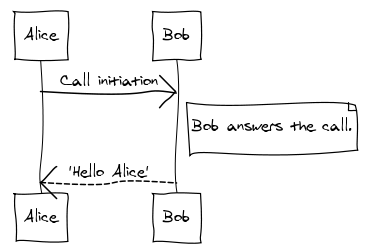
\includegraphics[width=9cm]{uml_seq_example.png}\\
  \caption[Example figure]{Alice and Bob}
  \label{fig:aliceandbob}
\end{figure}

\section{Results for Experiment B\label{sec:results2}}
In Table~\ref{table:example} the statistics for...

\begin{table}[H]
  \begin{center}
  \begin{tabular}{ | p {2.5cm}| p{3.6cm}| p{3.6cm}| p{3.3cm}| }
  \hline
  \textbf{Dateset} & \textbf{Minimum y} & \textbf{Maximum y} & \textbf{Average y} \\
  \hline
  DS 1 & -68.57 & 506.78 & 86.05 \\ \hline
  DS 2 & -0.18 & 537.67 & 102.51 \\
  \hline
  \end{tabular}
  \caption[Example table]{This table shows the statistics (minimum, maximum, and average) for the different datasets.}
  \label{table:example}
  \end{center}
\end{table}


\section{Discussion of Results\label{sec:resultDiscussion}}
...

    \chapter{Related Work\label{cha:chapter5}}

This chapter provides insights into additional related work that was not mentioned in the background chapter. 

    \chapter{Conclusions\label{cha:chapter6}}

This chapter summarizes the contriubtions of the thesis and provides an outlook into future work. 

% ---------------------------------------------------------------
\backmatter % no page numbering from here
    \addchap{List of Acronyms}

\begin{tabbing}
spacespacespace \= space \kill
ML	 \> 	Machine Learning	 \\
\end{tabbing}
\endinput

		
		% if you want to provide a glossary with explanations of important terms put it in here

    % \bibliographystyle{geralpha}
    % \bibliography{./bib/manual}
    \printbibliography  
    \addchap{Appendix}

\begin{appendix}

Add additional experimental results that do not need to be directly included in the thesis body. 

\end{appendix}

\endinput


\end{document}
